% !TEX encoding = UTF-8 Unicode
% !TeX spellcheck = en_US


% Latex-Template für die VDI Mechatroniktagung 2015
% Lehrstuhl für Regelungssystemtechnik, TU Dortmund
% Letzte Änderung: 18.02.2014

\documentclass[fleqn,a4paper,10pt]{article}

% Packages
\usepackage{mathptmx} % Times Schriftart (auch in der Math-Umgebung)
\usepackage[german, english]{babel}
\usepackage[utf8]{inputenc} % Deutsche Sonderzeichen/Umlaute gestatten
\usepackage[T1]{fontenc}
\usepackage[nooneline,bf,labelsep=quad,font=small]{caption} % Bildunterschrift linksbündig

\usepackage{multicol}

\usepackage{amsmath} % Zur Abbildung mathematischer Symbole und Formeln
\usepackage{amssymb}
\newcommand{\bm}[1]{\mathbf{#1}}
\renewcommand{\Phi}[1]{\varPhi{#1}}
\newcommand{\rotmat}[2]{{{ }^{#1}\bm{R}}_{#2}}
\newcommand{\ortvek}[4]{{ }_{(#1)}{\bm{#2}}^{#3}_{#4} }
\newcommand{\transp}[0]{{\mathrm{T}}}
\newcommand{\ks}[1]{{(\mathrm{CS})}_{#1}}
\usepackage[fleqn]{nccmath} % Ausrichtung von Gleichungen
\usepackage{paralist}
\usepackage{graphicx}
\usepackage{graphbox}   % allows to add keys to \includegraphics
\graphicspath{{./Bilder/}}
\usepackage{color}
\usepackage{geometry}

\usepackage{booktabs} % Erweiterte Tabellenumgebung
\usepackage{cite} % Erweitertes Zitiermöglichkeiten

\usepackage{titlesec} % Abstand vor und hinter Abschnittstiteln.

\usepackage{etoolbox} % Scriptsammlung. Z.B. horizontalen Abstand zwischen Literatureintrag und jeweiligem Label verändern.


% Seiteneinstellungen
\geometry{left=2.025cm, right=2cm, top=2.07cm, bottom=2.8cm} % Geringe Änderungen, um mit Word übereinzustimmen.
\parindent0cm
\columnsep5mm
\parskip 0pt   
\pagestyle{empty}                  % Kopf- und Fußzeile entfernen

% Abschnittsüberschriften
\captionsetup[table]{skip=-1.4ex} % Abstand zwischen Tabelle und Tabellenbeschriftung
\captionsetup[figure]{skip=5mm} % Abstand zwischen Bild und Bildunterschrift

% Paper-Titel
\titlespacing*{\section}{0pt}{6pt}{6pt}
\titlespacing*{\subsection}{0pt}{6pt}{6pt}
\titleformat{\section}{\normalfont\Large\bfseries}{\thesection\hskip 1cm}{0pt}{} % Abstand zwischen Titelnummer und Beschriftung.
\titleformat{\subsection}{\normalfont\large\bfseries}{\thesubsection\hskip 0.7cm}{0pt}{}

% Gleichungen
\setlength{\mathindent}{0.5cm} % Abstand von Gleichungen zum linken Rand.

% Tabelleneinstellungen
%\renewcommand{\arraystretch}{9.5} % Abstand zwischen Zeilen in einer Tabelle -> Steht in Vorlage, führt in Formel-Array zu sehr großem Abstand
\setlength{\tabcolsep}{6pt} % Abstand zwischen Spalten in einer Tabelle

% Umgebungsdefinitionen
\newenvironment{mytitle}{\fontsize{16pt}{1.0} \selectfont \bfseries}{\\} 
\newenvironment*{myabstract}{\begin{Large}\bfseries}{\end{Large}\\[6pt]}%

\renewenvironment{figure}
  {\par\vspace{6pt}\noindent\minipage{\linewidth}}
  {\endminipage\par\vspace{6pt}}


\renewenvironment{table}
  {\par\vspace{6pt}\noindent\minipage{\linewidth}\fontsize{8.5pt}{1.2} \selectfont}
  {\endminipage\par\vspace{6pt}}

\makeatletter

\g@addto@macro\normalsize{%        % Abstand vor und hinter Gleichungsumgebungen.
  \setlength\abovedisplayskip{6pt}
  \setlength\belowdisplayskip{6pt}
  \setlength\abovedisplayshortskip{6pt}
  \setlength\belowdisplayshortskip{6pt}
}

\makeatother

% Literaturverzeichnis
\patchcmd{\thebibliography}{\advance\leftmargin\labelsep}
  {\advance\leftmargin\labelsep \labelsep=0.4cm}{}{} % Horizontalen Abstand anpassen (etoolbox)
\patchcmd{\thebibliography}{\section*}{\section}{}{} % Abschnittsnummer hinzufügen

\let\OLDthebibliography\thebibliography % Vertikalen Abstand anpassen
\renewcommand\thebibliography[1]{
  \OLDthebibliography{#1}
  \setlength{\parskip}{0pt}
  \setlength{\itemsep}{2pt}
}


\begin{document}

\begin{mytitle}
\foreignlanguage{german}{
Maßsynthese für Parallele Roboter: Einheitliche Kinematik und\\ Dynamik mit vollständigen kinematischen Zwangsbedingungen} \\[6pt] % Falls Zeilenumbruch erforderlich, \\[6pt] anfügen.
Dimensional Synthesis of Parallel Robots: Unified Kinematics and\\ Dynamics using Full Kinematic Constraints
\end{mytitle}

Moritz Schappler, Prof. Dr.-Ing. Tobias Ortmaier, Leibniz Universität Hannover, Institut für Mechatronische Systeme, Appelstraße 11a, 30167 Hannover, Deutschland. Korrespondenz: moritz.schappler@imes.uni-hannover.de.

\vspace{24pt} % Bitte nicht entfernen.

\foreignlanguage{german}{
\begin{myabstract} Kurzfassung \end{myabstract}
Durch systematische Struktursynthese wurden bislang eine Vielzahl unterschiedlicher parallelkinematischer Maschinen (PKM) beschrieben. 
Um die passendste Roboterkinematik für eine gegebene Aufgabe zu finden, ist eine effiziente und allgemeingültige Auswahlsystematik erforderlich. 
Für einfache Systeme mit mehrwertigen Gelenken wie die Gough-Stewart-PKM liegen bereits Modellierungs- und Optimierungsverfahren vor. 
Für komplexere Strukturen mit mehr einwertigen Gelenken ist die Auswahl an Verfahren eingeschränkter. 
Der vorliegende Beitrag führt allgemeine Ansätze für die Modellierung der Kinematik und Dynamik zusammen, um die Maßsynthese von PKM besonders effizient zu gestalten.}


\vspace{12pt} % Bitte nicht entfernen.


\begin{myabstract} Abstract \end{myabstract}
A variety of different structures for parallel kinematic machines (PKM) have been found by means of systematic structural synthesis.
To find the structure that is suited best for a specific task, an efficient and generic selection method is necessary.
For simple structures with multi-degree-of-freedom joints like the Gough-Stewart robot, methods for modeling and dimensional optimization are well established.
Less methods are available for more complex structures with single-degree-of-freedom joints.
This contribution combines general approaches for the modeling of the kinematics and dynamics of parallel robots to obtain an efficient dimensional synthesis of PKM.

\vspace{18pt} % Bitte nicht entfernen.


\begin{multicols}{2}

\section{Introduction}

%\begin{itemize}
%\item Die Struktursynthese paralleler Roboter hat durch die systematische Nutzung der Schraubentheorie \cite{KongGos2007} und der evolutionären Morphologie \cite{Gogu2008} eine Vielzahl neuer Parallelkinematiken hervorgebracht, für die Großteils noch keine praktische Anwendung gefunden wurde, obwohl es bereits einige unterschiedliche PKM-Demonstratoren an Forschungseinrichtungen gibt \cite{Merlet2006}.
%\item Um für gegebene Anforderungen an einen Roboter den bestgeeignetsten auszuwählen, ist eine automatische Auslegung (Maßsynthese) notwendig, die für die Vielzahl verfügbarer Kinematiken anwendbar ist.
%%\item Der vorliegende Beitrag behandelt eine allgemeine Methodik für die Maßsynthese paralleler Kinematiken unter Ausnutzung struktureller Eigenschaften von Kinematik und Dynamik sowie der effizienten Strukturierung des Optimierungsproblems.
%\item Maßsynthese paralleler Roboter großer Schwerpunkt in den 2000er Jahren \cite{MbarekNefCor2005,Krefft2006,FrindtKreHes2010} durch Forschung deutscher Produktionstechnik-Instituten und internationen Forschungsgruppen \cite{CarboneOttCec2007,KelaiaiaComZaa2012,JamwalHusXie2015}
%\item Es wurde festgestellt, dass die theoretisch erreichbaren Eigenschaften von PKM wesentlich von der Auslegung der Maschinen abhängen und die Maßsynthese eine größere Rolle als bei seriellen Robotern einnimmt \cite{Merlet2006}
%\item Bisher hauptsächlich Fokus auf Klassischen PKM mit mehrwertigen Gelenken und wenigen Gliedern, da durch die technische Ausgestaltung eine hohe Steifigkeit erreicht werden kann, die für Bearbeitungsprozesse entscheidend ist \cite{MbarekNefCor2005}
%%\item Ursache ist die voraussichtlich niedrigere Steifigkeit und Kollisionsanfälligkeit von PKM mit mehrgliedrigen Beinketten
%\end{itemize}

The structural synthesis of parallel robots by means of screw theory \cite{KongGos2007} or evolutionary morphology \cite{Gogu2008} has produced a variety of different architectures.
However, for only few of them a specific application has been found despite numerous research demonstrators focusing on single aspects of the robots \cite{Merlet2006}.
It is well established that the theoretical advantages of parallel robots are strongly dependent on their dimensioning \cite{Merlet2006}. % and the dimensional synthesis has a more important role than for serial robots \cite{Merlet2006}.
An automatic dimensioning (i.e. dimensional synthesis) for all existing types of robots is necessary to select the robot that is suited best for a specific given application.
Therefore, the aspect of selecting a structure (structural synthesis) and choosing specific parameter values (dimensional synthesis) should be performed in a combined structural and dimensional synthesis \cite{Krefft2006}.
Efforts on the dimensional synthesis constitute a major part in the research of parallel robots, beginning in the early 2000s driven by international robotics research groups, e.g. \cite{Merlet2006,CarboneOttCec2007}, and German researchers in the field of machine tools, e.g. \cite{MbarekNefCor2005,Krefft2006,FrindtKreHes2010}.
Until today, research is focused mainly on parallel robots with leg chains with the minimal amount of links and joints with multiple degrees of freedom (DoF), like universal and spherical joints.
This has advantages for the stiffness, which is essential for machining tasks \cite{MbarekNefCor2005}.


%Quellen (z.B.)
%\cite{JamwalHusXie2015}
%
%\cite{CarboneOttCec2007}
%\cite{ZhouBaiHan2011}

%Einschränkungen Stand der Technik
%\begin{itemize}
%\item Maßsynthese in Beispielen häufig nur für einen Roboter durchgeführt z.B. Delta-Roboter \cite{KelaiaiaComZaa2012}, Gough-Stewart [Quelle], Hexa \cite{Krefft2006}, bislang in \cite{Krefft2006} als Ausblick beschriebene kombinierte Struktur- und Maßsynthese nur für serielle Roboter durchgeführt \cite{Ramirez2018}.
%\item Für PKM mit mehrgliedrigen Beinketten gibt es nicht immer eine analytische Lösung von Kinematik und Dynamik
%\item Auslegung wird überwiegend basierend auf kinematischer und kinetostatischer Merkmale ausgeführt \cite{CarboneOttCec2007} [...], die Dynamik wird nur selten betrachtet, z.B. durch die Berechnung einer minimal möglichen Beschleunigung basierend auf Antriebskräften und bewegte Masse \cite{Krefft2006}.
%Eine teilweise Betrachtung der Dynamik erfolgt durch die Konditionszahl der Massenmatrix in \cite{KelaiaiaComZaa2012} oder Eigenfrequenz berechnet aus Massen- und Steifigkeitsmatrix in \cite{JamwalHusXie2015}. Bei seriellen Robotern öfter Anwendung in Maßsynthese, z.B. durch Berechnung mit Adams \cite{ZhouBaiHan2011}
%\item Auswahl von Antrieben bisher hauptsächlich bei seriellen Robotern ein Thema, z.B. \cite{ZhouBaiHan2011} und nicht bei PKM, da Antriebe bei PKM klassischerweise Gestellfest angeordnet sind und die Auswahl wenig Rückwirkung auf den Roboter hat
%\item mehrkriterielle Pareto-Optimierung relativ stark verbreitet, z.B. durch Algorithmen Strength Pareto Evolutionary Algorithm \cite{Krefft2006,KelaiaiaComZaa2012},  nondominated sorting
%algorithm (NSGA II) \cite {JamwalHusXie2015} (angeblich besser). Mehrkriterielle Optimierung mit Gewichtung gilt als ineffizient \cite{JamwalHusXie2015}
%\item Keine systematische Berücksichtigung der Schnittkräfte mittels analytischer Modelle, nur mit FEM für serielle Roboter in wenigen Quellen, z.B. parametrisches CAD-Modell mit Ansys \cite{ZhouBai2015} und von-Mises Vergleichsspannung
%\end{itemize}

Only few authors report a dimensional synthesis for multiple different robots with the ambition to compare them by this means, e.g. \cite{Krefft2006} in a case study for two different architectures of Delta robots or \cite{Ramirez2018} for serial robots.
Most authors perform the dimensional synthesis for specific structures, such as the  Delta robot \cite{StockMil2003,KelaiaiaComZaa2012}, the Hexa robot \cite{Krefft2006}, the CaPaMan \cite{CarboneOttCec2007} or a cable-driven ankle rehabilitation robot \cite{JamwalHusXie2015}.
The synthesis is mainly focused on kinematic characteristics such as workspace and conditioning of the Jacobian or kinetostatic characteristics such as the stiffness \cite{CarboneOttCec2007,KelaiaiaComZaa2012}. % of the manipulator and its isotropy in the workspace and in different directions [].
The dynamics of the parallel robot is only regarded in some cases, e.g. by taking the minimal possible acceleration of the machine as a constraint \cite{Krefft2006}.
A partly consideration of dynamics aspects is performed by assessing the condition number of the mass matrix in \cite{KelaiaiaComZaa2012} or the Eigen frequencies of the robot obtained from the mass and stiffness matrix in \cite{JamwalHusXie2015}.
In the dimensional synthesis of serial robots more attention is paid to the dynamics equation, e.g. by \cite{ZhouBaiHan2011} using a multi-body simulation tool like \textsc{Adams} in the optimization loop.
%The selection of the drive train of the actuated joints, as e.g. treated in \cite{ZhouBaiHan2011} for serial robots, is rarely part of the synthesis of parallel robots, since the drives mounted at the robot base have little effect on the robot dynamics.
A consideration of material stress and internal forces is to the best knowledge of the authors only performed in the dimensional synthesis of serial robots, e.g. by \cite{ZhouBai2015} who perform FE analyses with \textsc{Ansys} for a parametric CAD model inside the optimization loop.

Usually, a heuristic multi-objective optimization is performed in the dimensional synthesis, e.g. with the Strength Pareto Evolutionary Algorithm \cite{Krefft2006,KelaiaiaComZaa2012} or the Nondominated Sorting Genetic Algorithm \cite{JamwalHusXie2015}.
Using a weighted sum to incorporate multiple objectives is prone to the subjectivity of the user \cite{JamwalHusXie2015}. % and may prevent a clear comparison of different arch  requires high effort in defining the weights and \cite{JamwalHusXie2015}
%The optimization with a weighted sum of different objectives is claimed to be insufficient by.
%Some groups also used algorithms like SQP \cite{CarboneOttCec2007}.


To be able to perform a dynamics-based optimization of general parallel robots without assumptions on the joint types, this paper addresses a general and efficient formulation of the optimization problem.
%To encounter possible gaps in the dimensional synthesis of parallel robots using dynamics-based criteria, this paper addresses a general and efficient formulation of the optimization problem which can be extended to all possible parallel robots without assumptions on the type of joints.
%This paper addresses the aspect of a combined dimensional synthesis using a dynamics-based criterion.
%
The contributions of the paper are
\begin{compactitem}
%\item Anwendung der allgemeinen PKM-Modellierung auf nicht-konventionelle PKM
%\item Vorschlag einer effizienten Optimierungsstruktur für die Maßsynthese von PKM
%\item Beispiele und simulative Validierung des Verfahrens
\item the application of a general kinematic and dynamics model on the dimensional synthesis of non-conventional parallel robots,
\item the proposition of an efficient optimization structure,
\item examples and simulative results.
\end{compactitem}

The remainder of the paper is structured as follows: The general model of the kinematics and dynamics is presented in Sec.\,\ref{sec:sysmdl}.
The structure for defining the optimization problem of dimensional synthesis is sketched in Sec.\,\ref{sec:opti} followed by the results in Sec.\,\ref{sec:results} and a summary in Sec.\,\ref{sec:summary}.

\section{System Description and Model}
\label{sec:sysmdl}

%\cite{Merlet2006}
%\cite{Gogu2008}
%\cite{BriotKha2015}


%\begin{itemize}
%\item Paralleler Roboter mit 6 FG, Plattform-Pose $\bm{x}$, translatorischer und rotatorischer Teil mit Euler-Winkeln
%\item $m$ Beinketten mit den Gelenkwinkeln $\bm{q}_1$, ..., $\bm{q}_m$ jeweils mit allen aktiven und passiven Gelenken inklusive der Koppelgelenke mit der Plattform
%\item Definition Koppelpunkte $A_i$ und $B_i$, Basis $O$ und Plattform $E$
%\item Schließung der kinematischen ZB über Zwangsbedingungen $\bm{\Phi}$ für gesamte PKM
%%\item Lösung des IKP für jede Beinkette einzeln. 
%\end{itemize}


The general parallel robot model subject to the dimensional synthesis in this paper consists of $m$ leg chains with $n_i$ joints each, which support the moving platform with respect to a fixed base.
A sketch of the robot is depicted in Fig.\,\ref{fig:PKM_kinematics} with the necessary coordinate systems (``CS'') for kinematic modeling, including a base frame $\ks{0}$ of the PKM and base frames $\ks{A_i}$ and virtual end effectors $\ks{E_i}$ for the leg chains.
The definition of the coupling frames $\ks{B_i}$ on the platform allow arbitrary alignments of legs and platform.
The moving platform frame $\ks{P}$ is expressed with the minimal coordinates $\bm{x}$ containing the Cartesian position $\bm{x}_\mathrm{t}$ and orientation  $\bm{x}_\mathrm{r}$ (as three Euler angles).
The joint coordinates $\bm{q}_i$ of each leg chain $i$ are stacked as
%
\begin{equation}
\bm{q}^\transp=(\bm{q}_{1}^\transp,\cdots,\bm{q}_{m}^\transp) \quad \mathrm{with}  \quad \bm{q}_i^\transp=(q_{i,1},\cdots,q_{i,n_i}).
\end{equation}

\begin{figure}
    \graphicspath{{./Bilder/}}
    \centering
    \input{Bilder/PKM_Kinematik.pdf_tex}
    \captionof{figure}{Sketch of the general parallel robot kinematics}
    \label{fig:PKM_kinematics}
\end{figure}


This general model extends the formulation in textbooks \cite{Merlet2006,BriotKha2015} by including coordinates of passive \emph{and} coupling joints to avoid assumptions on the solvability of the kinematic equations (``minimal kinematics set'', \cite{Merlet2006}).
%By defining the coupling as frame $\ks{B_i}$ instead of the position of the last joint of the leg chain, arbitrary alignments of the coupling joint can be realized.
%A set of kinematic constraints $\bm{\Phi}$ is used to close the kinematic loops w
The following sections introduce the unified kinematic (Sec.\,\ref{sec:kinematics}) and dynamics (Sec.\,\ref{sec:kindyn}) modeling, which leads to the calculation of internal forces (Sec.\,\ref{sec:intforce}) and energy (Sec.\,\ref{sec:energy}) used in the dimensional synthesis of parallel robots and sketched in Fig.\,\ref{fig:details_kindyn}.



\subsection{Full Kinematic Constraints}
\label{sec:kinematics}
%\cite{SchapplerTapOrt2019c}


%\begin{itemize}
%\item Zunächst werden die Gelenkgrößen $\bm{q},\dot{\bm{q}},\ddot{\bm{q}}$ des Roboters mittels der vollständigen \emph{inversen Kinematik} berechnet (linker Block in Bild\,\ref{fig:details_kindyn}).
%\item Die dafür notwendigen vollständigen kinematischen Zwangsbedingungen (``ZB'') $\bm{\Phi}$ enthalten für jede Beinkette sowohl den Positions-, als auch den in Euler-Winkeln ausgedrückten Orientierungsfehler \cite{SchapplerTapOrt2019c}.
%\item Definition der ZB mit Formeln
%\item Durch Bildung der Gradienten ($\bm{\Phi}_\bm{q}$ und $\bm{\Phi}_\bm{x}$) können mit der vollständigen Jacobi-Matrix $\tilde{\bm{J}}$ neben den aktiven Gelenkkoordinaten $\bm{q}_\mathrm{a}$ auch passive Gelenke und Schnittgelenke der Plattform berechnet werden, die gemeinsam in $\bm{q}$ zusammengefasst sind.
%\end{itemize}

To be able to solve the inverse kinematics problem for all active and passive joint coordinates $\bm{q}$, a full set of kinematic constraints has to be defined.
In the context of dimensional synthesis, a trajectory of the platform pose $\bm{x}(t)$ is given and has to be accomplished by the simulated parallel robot.
These constraints can e.g. be defined as vector loops between the respective leg chains \cite{Gogu2008} or one leg and the platform \cite{Merlet2006}.
The formulation of the full kinematic constraints on position level instead of velocity level has the advantage of providing a feasible residual for a gradient-based solution of the inverse kinematics problem \cite{SchapplerTapOrt2019c}. %, as presented by the authors in . 
%
%able to solve the inverse kinematics problem 
The translational part of the full kinematic constraints can be formulated as the difference of the coupling point position $B_i$ on the platform and the corresponding coupling joint $E_i$ on the leg chain $i$ with

%For a parallel robot with full mobility, three translational

%
\begin{equation}
\bm{\Phi}_{\mathrm{t},i}(\bm{q}_i,\bm{x}) = - \bm{r}_{A_iB_i}(\bm{x}) + \bm{r}_{A_iB_i}(\bm{q}_i)
\overset{!}{=} \bm{0},
\label{equ:kinconstrAB}
\end{equation}
%
as established in the state of the art \cite{Merlet2006} and sketched in Fig.\,\ref{fig:PKM_kinematics}.
The minimal form of the rotational part of the kinematic constraints is calculated with the Euler angles $\bm{\phi}_{XYZ}$ of the rotational difference of the frames $\ks{E_i}$ on the leg chain $i$ and the corresponding $\ks{B_i}$ on the platform, with
%
\begin{align}
\bm{\Phi}_{\mathrm{r},i}(\bm{q}_i,\bm{x})
=
\bm{\phi}_{XYZ}\left(\rotmat{0}{B_i}^\transp (\bm{x}_{\mathrm{r}})\rotmat{0}{E_i}(\bm{q}_i)\right)
\overset{!}{=} \bm{0},
\label{equ:Phir_def_i}
\end{align}
%
as elaborated in detail in \cite{SchapplerTapOrt2019c}.
%
The kinematic constraints for the whole robot are then stacked with the terms for the single leg chains to 
%
\begin{equation}
\bm{\Phi}^\transp
=
(\bm{\Phi}_1^\transp,
\cdots,
\bm{\Phi}_m^\transp
),
\quad
\mathrm{with}
\quad
\bm{\Phi}_i^\transp=(
\bm{\Phi}_{\mathrm{t},i}^\transp, \bm{\Phi}_{\mathrm{r},i}^\transp
).
\label{equ:constr_Phi_PKM}
\end{equation}

The full inverse Jacobian of the parallel robot
%
\begin{equation}
\tilde{\bm{J}}^{-1}=-\left( \frac{\partial \bm{\Phi}}{\partial \bm{q}} \right)^{-1} \left( \frac{\partial \bm{\Phi}}{\partial \bm{x}} \right)
\quad \mathrm{with} \quad
\dot{\bm{q}}=\tilde{\bm{J}}^{-1} \dot{\bm{x}}% , \quad
%\quad \mathrm{and} \quad 
%\bm{\Phi}_{\bm{q}}=\frac{\partial \bm{\Phi}}{\partial \bm{q}}
\label{equ:jacobian}
\end{equation}
%
is obtained by time differentiation of the constraint equation (\ref{equ:constr_Phi_PKM})  and relates the velocities $\dot{\bm{q}}$ of all joints and the platform $\dot{\bm{x}}$.
To extract only the velocity $\dot{\bm{q}}_\mathrm{a}$ of the actuated joints, the corresponding rows in $\dot{\bm{q}}$ are extracted with the selection matrix $\bm{P}_{\mathrm{a}}$ with
%
\begin{equation}
\bm{q}_{\mathrm{a}} = \bm{P}_{\mathrm{a}} \bm{q}
\quad \mathrm{and} \quad
\bm{J}^{-1}=\bm{P}_{\mathrm{a}} \tilde{\bm{J}}^{-1},
\label{equ:jacobian_actuation}
\end{equation}
%
giving the analytic Jacobian of the parallel robot, which is square for non-redundant robots. % and subject to investigations known from literature \cite{Merlet2006}.
The joint accelerations can be obtained by differential calculus as
%
\begin{equation}
\ddot{\bm{q}}=\tilde{\bm{J}}^{-1}\ddot{\bm{x}}+\dot{\tilde{\bm{J}}}^{-1}\dot{\bm{x}}.
\label{equ:acceleration_jacobian}
\end{equation}
%
The partial derivatives in (\ref{equ:jacobian}) can be partly  calculated in analytic form, as described in \cite{SchapplerTapOrt2019c}.
The inversion of the $36 \times 36$-matrix $\partial \bm{\Phi} / \partial \bm{q}$ (in the full-mobility case) should be performed numerically.
The derivatives of the terms required for (\ref{equ:acceleration_jacobian}) can also be partly calculated symbolically.

For an efficient calculation of the whole robot trajectory for time step $k$ with $t=k \Delta t$ with $k=1,...,n_t$, the kinematic relation
%
\begin{equation}
\bm{q}_{k+1}=\bm{q}_k+\dot{\bm{q}}_k \Delta t+\frac{1}{2}\ddot{\bm{q}}_k\Delta t^2
\label{equ:IK_initialvalue}
\end{equation}
%
can be used as an initial value for the gradient-based solution of the inverse kinematics problem \cite{KhalilDom2002},\cite{SchapplerTapOrt2019c}.

\subsection{Unified Kinematics and Dynamics}
\label{sec:kindyn}

\begin{figure*}[b]
    \centering
    \input{./Bilder/Details_Kin_Dyn.pdf_tex}
    \captionof{figure}{Unified calculation of the inverse kinematics and inverse dynamics for application in the dimensional synthesis}
    \label{fig:details_kindyn}
\end{figure*}

%, (\ref{equ:invdyn_leg}), (\ref{equ:coupling_wrench_leg}), (\ref{equ:intforce_fromcoupling}),

%Für die Bestimmung des Energieverbrauchs für eine Referenztrajektorie wird ein allgemeingültiger Ansatz für die \emph{inverse Dynamik} beliebiger paralleler Roboter benötigt.
%Das zu diesem Zweck in \cite{AbdellatifHei2009,DoThanhKotHeiOrt2009b} vorgestellte Prinzip der Energieäquivalenz wird dafür erweitert.
%Zunächst erfolgt die Zerlegung des parallelen Roboters in einzelne Subsysteme (Beinketten und Plattform), in deren jeweiligen Minimalkoordinaten (Gelenk- und Plattformkoordinaten) die Dynamik einzeln nach dem \textsc{Lagrange}schen Formalismus aufgestellt wird (vollständige Massenmatrix $\tilde{\bm{M}}$, Coriolis- und Fliehkraftterme $\tilde{\bm{c}}$, Gravitationsterme $\tilde{\bm{g}}$) \cite{DoThanhKotHeiOrt2009b}.
%Anschließend erfolgt die Projektion der Dynamik in die Minimal-/Plattformkoordinaten $\bm{x}$ des Roboters durch Anwendung des \textsc{D'Alembert}schen Prinzips, woraus die Dynamik-Terme $\bm{M},\bm{c},\bm{g}$ bezogen auf die Plattform resultieren \cite{DoThanhKotHeiOrt2009b,AbdellatifHei2009} (siehe mittlerer Block in Bild\,\ref{fig:details_kindyn}).
%Die Jacobi-Matrix $\tilde{\bm{J}}$ aus der inversen Kinematik kann direkt ohne Neuberechnung für die Dynamik-Projektionsmatrix $\tilde{\bm{D}}$ eingesetzt werden.
%Durch die Verwendung rotatorischer Zwangsbedingungen \cite{SchapplerTapOrt2019c} zusätzlich zu den translatorischen Zwangsbedingungen kann die implizite Annahme aus \cite{AbdellatifHei2009} aufgehoben werden, dass die Beinketten räumlicher Parallelkinematiken in Kugelgelenken enden müssen.
%Diese Bedingung wird z.\,B. von einigen der durch Gosselin et al. \cite{KongGos2007} und Gogu et al. \cite{Gogu2008} erzeugten Roboter nicht erfüllt.

To be able to determine the energy consumption of an arbitrary parallel robot for the reference trajectory of the dimensional synthesis, the inverse dynamics is required.
The application of the principle of energy equivalence for parallel robots from \cite{AbdellatifHei2009,DoThanhKotHeiOrt2009b} has to be extended using the full kinematic constraints from the previous section.
The formulation from Abdellatif et al. \cite{AbdellatifHei2009} only applies for parallel robots which can be described solely with translational constraints (\ref{equ:kinconstrAB}), i.e. robots with leg chains containing at most two links and end in spherical joints in the full mobility case.
Some of the the robots resulting from the structural synthesis from Gosselin et al. \cite{KongGos2007} and Gogu et al. \cite{Gogu2008} do not meet this requirement.

Following the more general approach from Do Thanh et al. \cite{DoThanhKotHeiOrt2009b} the parallel robot is decomposed into the subsystems leg chains and platform.
The inverse dynamics for the subsystems in their respective minimal coordinates $\bm{q}_i$ and $\bm{x}$ can be obtained with standard methods such as the \textsc{Lagrange} equations.
The resulting terms of the explicit dynamics equation can be assembled as the block diagonal of the full inertia matrix $\tilde{\bm{M}}$ and stacked as the full Coriolis and centrifugal forces vector $\tilde{\bm{c}}$ and gravitational forces vector $\tilde{\bm{g}}$.
The implicit form $\tilde{\tau}$ of the dynamics can be assembled as the sum of the single terms as
\begin{equation}
\tilde{\tau} = \tilde{\bm{M}} [\ddot{\bm{q}}^\transp, \ddot{\bm{x}}^\transp]^\transp + \tilde{\bm{c}} + \tilde{\bm{g}}.
\label{equ:subsys_implicit_dyn}
\end{equation}

%, can be stacked in $\tilde{\bm{M}}$, $\tilde{\bm{c}}$, $\tilde{\bm{g}}$ and $\tilde{\bm{\tau}}$, $\tilde{\tau}$

By applying the principle of \textsc{D'Alembert}, the dynamics of the subsystems can be projected into the minimal coordinates $\bm{x}$ of the parallel robot.
To this end, the Jacobian matrix from the inverse kinematics step in (\ref{equ:jacobian}) is extended by a unit matrix corresponding to the platform coordinates to obtain the projection matrix
%
\begin{equation}
\tilde{\bm{D}}^\transp=\left(\tilde{\bm{J}}^{-\transp},\bm{1}\right).
\label{equ:dyn_projection_matrix}
\end{equation}
%
The projection of the dynamics %corresponds to the constraint, closed-loop system and 
 gives
%
\begin{equation}
\bm{M}=\tilde{\bm{D}}^\transp\tilde{\bm{M}}\tilde{\bm{D}}, \quad
\bm{c}=\tilde{\bm{D}}^\transp (\tilde{\bm{M}}\dot{\tilde{\bm{D}}}\dot{\bm{x}}+\tilde{\bm{c}}),
\label{equ:invdyn_Mc}
\end{equation}
%
\begin{equation}
\bm{g}=\tilde{\bm{D}}^\transp\tilde{\bm{g}} \quad \mathrm{and} \quad 
\bm{\tau}=\tilde{\bm{D}}^\transp\tilde{\bm{\tau}}.
\label{equ:invdyn_gtau}
\end{equation}

%The Jacobian matrix from the inverse kinematics step in (\ref{equ:jacobian}) can be used directly to obtain the projection matrix
%%
%\begin{equation}
%\tilde{\bm{D}}^\transp=\left(\tilde{\bm{J}}^{-\transp},\bm{1}\right).
%\label{equ:dyn_projection_matrix}
%\end{equation}
%
To reduce the computational effort, the implicit form $\bm{\tau}$ of the inverse dynamics in (\ref{equ:invdyn_gtau}) should be used, avoiding the explicit computation of the inertia and Coriolis terms in (\ref{equ:invdyn_Mc}), which are not used in the dimensional synthesis, unless investigations on inertial forces \cite{FrindtKreHes2010} or Eigen frequencies \cite{JamwalHusXie2015} require the inertia matrix $\bm{M}$.
Further, this allows neglecting the matrix $\dot{\tilde{\bm{J}}}^{-1}$ in (\ref{equ:acceleration_jacobian}), which has low influence on the kinematics.
The actuator force for the calculation of the power consumption of the parallel robot are obtained with the inverse Jacobian from (\ref{equ:jacobian_actuation}) to

\begin{equation}
\bm{\tau}_\mathrm{a}
=\bm{J}^{-\transp} (\bm{M}\ddot{\bm{x}}+\bm{c}+\bm{g})
=\bm{J}^{-\transp} \bm{\tau}.
\label{equ:actforce}
\end{equation}

\subsection{Discussion on Velocity Constraints}

Using \textsc{D'Alembert}'s principle (``virtual work''), as proposed in \cite{DoThanhKotHeiOrt2009b} requires the definition of kinematic constraints at the position level, which demands some additional efforts for the orientation \cite{SchapplerTapOrt2019c}.
By defining the constraints on velocity level \cite{Gogu2008}, the calculation of the Jacobian is simplified by being able to use angular velocities and corresponding geometric Jacobians instead of Euler angles and their gradient matrices \cite{SaminFis2013}.
The dynamics are then effectively obtained with \textsc{Jourdain}'s principle (``virtual power''), leading to the same result.

\subsection{Internal Forces in Parallel Robots Legs}
\label{sec:intforce}

For an evaluation of the mechanical stress in the structure of the parallel robots legs, the internal forces and moments have to be known.
The projection-based dynamics does not produce cutting forces, since they do not perform work.
Using the Newton-Euler algorithm would provide these forces, but requires setting up a system of equations, which may be less generic than the projection approach.

The internal forces can be reconstructed by adapting the procedure presented in \cite{KhalilGue2004}.


\begin{figure}
\centering
\input{./Bilder/PKM_internal_forces.pdf_tex}
\captionof{figure}{Internal forces in the leg chains of the parallel robot}
\label{fig:PKM_internal_forces}
\end{figure}

With the known joint velocity $\dot{\bm{q}}_i$ and acceleration $\ddot{\bm{q}}_i$ from (\ref{equ:jacobian}) and (\ref{equ:acceleration_jacobian}) for all active and passive joints of the leg chain $i$, the stacked internal forces and moments
%
\begin{equation}
\bm{w}_{i,\mathrm{int}}=\bm{w}_{i,\mathrm{int}}(\bm{q}_i,\dot{\bm{q}}_i,\ddot{\bm{q}}_i)
\label{equ:intforce_leg}
\end{equation} % =\begin{pmatrix}\bm{w}_{i,\mathrm{int},0}^\transp & \cdots & \bm{w}_{i,\mathrm{int},n_i}^\transp\end{pmatrix}^\transp
%
can be computed with the recursive Newton-Euler algorithm for serial link kinematics \cite{KhalilDom2002,SaminFis2013}.
As sketched in Fig.\,\ref{fig:PKM_internal_forces}, the single leg chain $i$ cut open can be regarded as a serial link chain with an external wrench $\bm{w}_{B_i}$ acting at the last joint, giving the dynamics equation
 %
\begin{equation}
\bm{\tau}_i
=\bm{M}_i \ddot{\bm{q}}_i + \bm{c}_i + \bm{g}_i
=\bm{\tau}_{\mathrm{m},i} + \bm{J}_{i}^{\transp} \bm{w}_{B_i}.
\label{equ:invdyn_leg}
\end{equation}
%
The Jacobian $\bm{J}_{i}$ projects the external wrench (from perspective of the cut open leg chain) into the joint space coordinates $\bm{q}_i$ of the leg chain.
By assuming no kinematic redundancy and singularity, the equation can be rewritten to
%
\begin{equation}
\bm{w}_{B_i}=\bm{J}_{i}^{-\transp} (\bm{\tau}_i - \bm{\tau}_{\mathrm{m},i}),
\label{equ:coupling_wrench_leg}
\end{equation}
%
yielding the cut force and moment $\bm{w}_{B_i}$ in the coupling point $B_i$.
The motor torque $\bm{\tau}_{\mathrm{m},i}$ in the leg chain has zeros for passive joints and the corresponding entry $\bm{\tau}_{\mathrm{a},i}$ from (\ref{equ:actforce}).

\begin{equation}
\bm{w}_{i,\mathrm{coupl}}=\bm{J}_{i,\mathrm{full}}^{\transp} \bm{w}_{B_i}
\label{equ:intforce_fromcoupling}
\end{equation}


\begin{equation}
\bm{w}_{i} = -\bm{w}_{i,\mathrm{coupl}} + \bm{w}_{i,\mathrm{int}}
\label{equ:intforce_total}
\end{equation}

\subsection{Energy Consumption}
\label{sec:energy}

It is assumed that all electric drives of the actuated joints can exchange power in a common DC link, which is the case for newly installed robots, and enables improving energy efficiency in industrial production.
The mechanical power of the single robot actuators can be summed up (assuming no losses) to the electric DC link power
%
\begin{equation}
P_{\mathrm{link}}=\bm{\tau}_\mathrm{a}^\transp \dot{\bm{q}}_\mathrm{a}.
\label{equ:power_link_mech}
\end{equation}
%
Assuming no energy storage or recuperation, the electric power required from the grid results to
%
\begin{equation}
P_{\mathrm{grid}}=\left\{\begin{array}{ll} P_{\mathrm{link}}, & P_{\mathrm{link}}>0 \\0, & \mathrm{otherwise.}\end{array}\right.
\label{equ:power_link_grid}
\end{equation}
%
By integrating the power over time with
%
\begin{equation}
E_{\mathrm{grid}}=\int_{0}^{T_\mathrm{Traj}} P_{\mathrm{grid}} \, \mathrm{d}t
\label{equ:energy_integral}
\end{equation}
%
the energy consumption of the parallel robot in the reference trajectory can be obtained.

\section{Optimization}
\label{sec:opti}

The dimensional synthesis of parallel robots is implemented as a global optimization of the kinematic parameters of the robot.
As reasoned in \cite{JamwalHusXie2015,Ramirez2018}, performing a multi-objective optimization requires selecting a solution on the Pareto hyper-surface of all different objective criteria.
When trying to select the best robot architecture from many possibilities for a given task, an unambiguous criterion has to be used, not requiring a human decision \cite{Ramirez2018} or trial-and-error on weighting factors of different criteria \cite{JamwalHusXie2015}.
Therefore, a single-objective optimization is performed, where the energy consumption is used as an exemplary criterion and different constraints are used.
The particle swarm optimization is employed since it has, together with the genetic algorithm, proven to be efficient for this kind of design problem.
In the following, the problem formulation is elaborated in Sec.\,\ref{sec:opt_formulation}, the definition of the robot parameters is described in Sec.\,\ref{sec:opt_params} and the objective function and the various constraints are defined in Sec.\,\ref{sec:opt_objective} and Sec.\,\ref{sec:opt_constraints}.


\subsection{Formulation of the Problem}
\label{sec:opt_formulation}

\begin{figure*}

\centering
\input{./Bilder/optimization_overview.pdf_tex}
\captionof{figure}{Overview of the PSO optimization and the structure of the fitness function with hiearchichal constraints.}
\label{fig:uebersicht}
\end{figure*}

The ambition of the design optimization is to find the set of robot parameters (``particle'') $\bm{p}_\mathrm{opt}$, which minimizes the fitness function $f(\bm{p})$, leading to an optimal design.
Many parameter combinations however do not present a valid solution, since they violate some constraint.
Since the bottleneck in the optimization process is the computation time, an efficient way of handling the constraints is to abort the processing of a particle once one of the constraints is not met.
Therefore, from the different possibilities of including constraints in the optimization \cite{Jordehi2015}, an adaption of the static penalty approach is used which can be termed as ``hierarchical constraints''.
Following \cite{Ramirez2018}, the penalty terms $v_i$ are defined hierarchically according to the infeasibility of the solution with
%
\begin{equation}
v_1(\bm{p})>v_2(\bm{p})>\dots>z(\bm{p}),
\end{equation}
%
where $z$ represents the objective function and $v_i$ the penalty terms for the constraints, which are included in the piece-wise definition of the fitness function $f$, depicted in Fig.\,\ref{fig:uebersicht}.

To increase the convergence of the optimization as opposed to  constant penalties e.g. used in \cite{Ramirez2018}, the degree of violation $\rho>0$ of the constraints is included in the penalties $v_i$ and normalized with the function
%
\begin{equation}
f_\mathrm{norm}(\rho) = \frac{2}{\pi} \mathrm{arctan}(\rho / \rho_{\mathrm{scale}})
%\quad \mathrm{with} \quad
%0 < f_\mathrm{norm}(\rho) < 1
\label{equ:fnorm}
\end{equation}
%
to the range of $0$ to $1$.
Since it is not always possible to determine the upper limit of $\rho$ for any kind of parameter values, the saturation of (\ref{equ:fnorm}) ensures that each constraint penalty $v_i$ has a dedicated range in the possible values for the fitness function $f$.
The scaling $\rho_{\mathrm{scale}}$ adjusts the range of the values of $\rho$ which lie in the saturation of $f_\mathrm{norm} \approx 1$.
%By multiplying (\ref{equ:fnorm}) with a different factor, each constraint penalty $p_i$ has a dedicated range in the possible values for the fitness function $f$.


%Zur effizienten Berücksichtigung von Nebenbedingungen werden diese hierarchisch berechnet und normierte Strafterme $s_i$ direkt in der stückweise definierten Fitness-Funktion $f$ eingesetzt.
%Als skalare Zielfunktion $z$ wird der Energieverbrauch des Roboters über eine Referenz-Trajektorie $\bm{x}(t)$ gewählt, was einen direkten Vergleich unterschiedlicher Kinematiken erlaubt.
%Des Weiteren wird eine Korrelation mit anderen Zielfunktionen wie Gesamtmasse des Systems oder der Gleichförmigkeit der Eigenschaften (Konditionszahl der Jacobi-Matrix) erwartet.
%Die hierarchische Eigenschaft wird durch die Bedingung  und eine Normierung umgesetzt.


%Eine analytische Elimination der passiven Gelenke ist nicht für alle automatisch synthetisierten Strukturen aus möglich.
%Zusätzlich wird ein effizienter und allgemeingültiger Ansatz für die Dynamik benötigt.
%Der in Bild\,\ref{fig:details_kindyn} dargestellte und im Folgenden skizzierte  Ansatz erfüllt diese Anforderungen.






\subsection{Definition of Parameters}
\label{sec:opt_params}

To reduce the nonlinearity of the fitness $f$ function with respect to the optimization parameters $\bm{p}$, a conversion between optimization parameters and physical kinematic parameters of the robot is performed.
The measure especially aims at reducing the coupling between parameters.
Therefore, the following meta-parameters of the optimization are introduced:
\begin{compactitem}
\item the scaling parameter $p_\mathrm{scale}$ increases the size of the whole robot without changing its characteristics,% as far as possible,
\item the platform scaling parameter $p_\mathrm{plfscale}$ scales the diameter of the moving platform relative to the base.
\end{compactitem}

The kinematic parameters of the parallel robots are
%
\begin{compactitem}
\item the base diameter $d_\mathrm{base}=p_\mathrm{scale} p_\mathrm{base}$,
\item the platform diameter $d_\mathrm{plf}=p_\mathrm{plfscale} d_\mathrm{base}$,
\item the distance $d_\mathrm{basepairdist}=d_\mathrm{base} p_\mathrm{bpdscale}$ of coupling point pairs, in case of a pair-wise alignment at the base (Fig.\,\ref{fig:ergebnisse},a)
\item the pair distance $d_\mathrm{plfpairdist}=d_\mathrm{plf} p_\mathrm{ppdscale}$ for the moving platform (Fig.\,\ref{fig:ergebnisse},a,b),
\item the elevation $\alpha_\mathrm{Pyr}$ of the coupling joint, in case of a pyramidal alignment of the first joint axis of the leg chains (Fig.\,\ref{fig:ergebnisse},a,b),
\item the \textsc{Denavit-Hartenberg}-parameters for links $1\le i \le n_i$, $\alpha_{i,\mathrm{DH}}=p_{\alpha_i}$, $a_{i,\mathrm{DH}}=p_\mathrm{scale} p_{a_i}$, $\theta_{i,\mathrm{DH}}=p_{\theta_i}$ and $d_{i,\mathrm{DH}}=p_\mathrm{scale} p_{d_i}$, describing the serial link leg chains kinematics.
\end{compactitem}
%
Depending on the base and platform morphology (circular, pair-wise, pyramidal) and the kinematics of the symmetric legs, a different number of kinematic parameters
%
\begin{equation}
\bm{p}_\mathrm{kin}=[d_\mathrm{base}, d_\mathrm{plf}, d_\mathrm{basepairdist}, \cdots, d_{{n_i},\mathrm{DH}} ]^\transp % alpha_\mathrm{Pyr}, \alpha_{i,\mathrm{DH}},a_{i,\mathrm{DH}}, \theta_{i,\mathrm{DH}}
\end{equation}
%
and corresponding optimization parameters
%
\begin{equation}
\bm{p}=[p_\mathrm{scale}, p_\mathrm{base}, p_\mathrm{plfscale}, p_\mathrm{bpdscale}, \cdots, p_{d_{n_i}}]^\transp
\end{equation}
%
are subject to the optimization.

\subsection{Objective Function}
\label{sec:opt_objective}

Since the energy consumption of the parallel robot for a reference trajectory is a scalar value and is correlated with other criteria such as moved mass and joint speeds, it is a good candidate for an objective function of the dimensional synthesis.
The range of values for the energy from (\ref{equ:energy_integral}) is not known in advance.
The objective function
%
\begin{equation}
z=f_\mathrm{norm}(E_{\mathrm{Netz}})
\end{equation}
%
is therefore constructed by normalizing and saturating the energy value with the function from (\ref{equ:fnorm}).


%Für die Berechnung der \emph{Energie als Zielfunktion} (rechter Block in Bild\,\ref{fig:details_kindyn}) erfolgt eine Projektion der Dynamik auf die Antriebskräfte $\bm{\tau}_\mathrm{a}$. 
%Für die dafür notwendige Jacobi-Matrix $\bm{J}$ müssen lediglich die entsprechenden Spalten aus $\tilde{\bm{J}}$ gewählt werden.
%Es wird angenommen, dass alle Antriebe ihre Leistung in einem elektrischen Zwischenkreis austauschen können (resultierend zu $P_\mathrm{Kreis}$), was einem zukünftigen Szenario zur Erhöhung der Energieeffizienz entspricht.
%Für die aus dem Netz aufzunehmende Leistung $P_\mathrm{Netz}$ wird die Möglichkeit einer  Rückspeisung ausgeschlossen.
%Aus der aufintegrierten Energie $E_\mathrm{Netz}$ wird durch eine Normierung $f_\mathrm{norm}(\cdot)$ (mittels arctan-Funktion) der Zielfunktionswert $z$ gebildet.


\subsection{Constraints}
\label{sec:opt_constraints}

As introduced in Sec.\,\ref{sec:opt_formulation}, a hierarchy of constraints is assumed \cite{Ramirez2018} which extends the classical problem formulation in constrained optimization, where all constraints are handled equally as equality or inequality constraints \cite{Jordehi2015}.

\subsubsection{Geometric Feasibility}

First, the geometric feasibility of the parallel robot kinematic parameters is tested.
If the legs are too short to close the distance between base and platform radius, the first constraint penalty $v_\mathrm{leglength}$ is set.
If the coupling point $B_i$ is not reachable with the maximum length of a leg chain for any corner point of the workspace, the second penalty $v_\mathrm{cplreach}$ is set to a value corresponding to the longest missing leg length.

\subsubsection{Inverse Kinematics of Points and Trajectory}

Next, the inverse kinematics is solved for all corner points of the workspace.
The mean remaining violation of the kinematic constraints of (\ref{equ:constr_Phi_PKM}) serves as a penalty $v_\mathrm{IKcorner}$.
If this remains below the tolerance, i.e. all corner points are reachable, the inverse kinematics for the reference trajectory is calculated according to the left part of Fig.\,\ref{fig:details_kindyn}.
The first erroneous trajectory sample $k_{\mathrm{err}}$ in relation to the trajectory length $n_t$ serves as a penalty value $v_\mathrm{IKtraj}$.

\subsubsection{Joint Limits: Range, Velocity, Configuration}

For the given joint trajectory $\bm{q}(t)$ constraints on the feasibility regarding joint motion are checked.
First, limits on the joint range %$\mathrm{max\bm{q}_\mathrm{min} < \bm{q} < \bm{q}_\mathrm{max}$ are checked and the amount of exce
%
\begin{equation}
\bm{q}_\mathrm{range} = \max\limits_{t} \bm{q}(t) - \min\limits_{t} \bm{q}(t)
\label{equ:joint_range}
\end{equation}
%
are checked, where for revolute joints the $2\pi$-periodicity is regarded with an extended algorithm for (\ref{equ:joint_range}).
The allowed range of motion $\bm{q}_\mathrm{range,max}$ of revolute joints can be set lower for universal and spherical joints than for single-DoF revolute joints.
The maximum exceedance relative to the respective range results in the penalty term $v_\mathrm{jointrange}$.
%
Exceeding the maximum joint velocity $\dot{\bm{q}}_\mathrm{max}$ results in the penalty $v_\mathrm{jointvelo}$ and already indicates a bad-conditioned Jacobian.
%
Since a flipping of joint configurations (``elbow up/down'') can not be completely prevented in the gradient-based inverse kinematics, despite the initial value from (\ref{equ:IK_initialvalue}), the difference between the numeric differentiation of the joint positions $\bm{q}(t)$ from  and the velocities from the Jacobian in (\ref{equ:jacobian}) are taken as a penalty $v_\mathrm{configflip}$.

%\begin{equation}
%f_{\mathrm{jspeed},k} = \max\limits_{t}(\dot{q}_k(t)) / \dot{q}_{k,\mathrm{max}}
%\end{equation}
%\begin{equation}
%v_{\mathrm{jspeed}} = f_\mathrm{Norm}(\max\limits_{k} f_{\mathrm{jspeed},k}-1)
%\end{equation}

\subsubsection{Condition Number of the Jacobian}

If the joint trajectory has proven valid in the previous steps, the condition number of the Jacobian from (\ref{equ:jacobian_actuation}) is calculated for the trajectory.
If the condition number for any sample of the trajectory exceeds a threshold value, this indicates high actuator velocities or forces and leads to the penalty
%
\begin{equation}
v_{\mathrm{cond}} = f_\mathrm{norm}(\mathrm{log}[\max\limits_{t}  \mathrm{cond}(\bm{J}(t))]). % /k_{\mathrm{cond}}
\end{equation}
%
%where the scaling $k_{\mathrm{cond}}$ serves to adjust the range of condition numbers which lie in the saturation of $f_\mathrm{norm} \approx 1$.


\begin{figure*}[b]
\centering
\input{./Bilder/Optimierung_Ergebnisse.pdf_tex}
\captionof{figure}{Results of the dimensional synthesis of four robots with objective function $E_\mathrm{grid}$ and number of parameters $\mathrm{dim}(\bm{p})$.}
\label{fig:ergebnisse}
\end{figure*}

\subsubsection{Material Stress from Internal Forces}

To ensure a valid solution from the point of robot dynamics, internal forces in the leg chains are calculated according to Sec.\,\ref{sec:intforce}.
The force and moment in link $j$ of leg chain $i$ are combined in the wrench vector $\bm{w}_{i,j}^\transp=[\bm{f}_{i,j}^\transp, \bm{m}_{i,j}^\transp]$, as depicted in Fig.\,\ref{fig:PKM_internal_forces}.
The location of the maximum mechanical stress of each link is assumed to be proximal to the base and is calculated, simplified by neglecting torsional and shear stress, with 
%
\begin{equation}
\sigma_{i,j} = \max\limits_{t} \lVert\bm{f}_{i,j}\rVert / A_0 + \lVert\bm{m}_{i,j}\rVert / W,
\end{equation}
%
where $A_0$ is the sectional area and $W$ the resistance moment of the link structure, which is assumed to be a hollow cylinder.
The number
%
\begin{equation}
f_\mathrm{stress} = \max\limits_{i,j} \frac{\sigma_{i,j}}{\sigma_{\mathrm{max}}} % \max\limits_{i \in \{1,..m\}} \max\limits_{j \in \{1,..n_i\}}
\end{equation}
%
describes the maximum relative exceedance of the yield stress $\sigma_{\mathrm{max}}$ of the material for all links of the parallel robot and results in the penalty value
%
\begin{equation}
v_{\mathrm{stress}} = f_\mathrm{Norm}(f_\mathrm{stress}-1)
\quad \mathrm{for} \quad 
f_\mathrm{stress} > 1.
\end{equation}


\section{Simulation Results}
\label{sec:results}

%Hier nur Einleitungstext:
%\begin{itemize}
%\item Beispielhafte Durchführung der Maßsynthese für zwei Roboterkinematiken in zwei Varianten (siehe Ergebnisbild)
%\item Prinzipielle Funktionsweise des vorgestellten Ansatzes und qualitative Ergebnisse werden gezeigt
%\item Parametrierung der Struktursegmente als Hohlzylinder mit Parameter ..., Plattform als Kreisscheibe (Aluminium-Legierung Materialparameter)
%\item Detaillierte Betrachtung der Ergebnisse hinsichtlich Vorstellung der Roboter \ref{sec:res_scenario}, Funktionalität der hierarchischen Nebenbedingungen in \ref{sec:res_convergence}, Prüfung der vermuteten Notwendigkeit der Betrachtung von Materialspannung in \ref{sec:res_matstress}, Schwenkwinkel in \ref{sec:res_condition_pivoting}
%\end{itemize}

In the following, first simulative results for the optimization scheme from Sec.\,\ref{sec:opti} are presented.
The dimensional synthesis of two architectures of parallel robots with full mobility in two variants each is performed.
A detailed description of the simulation scenario and the robot parametrization is presented in Sec.\,\ref{sec:res_scenario}.
The functionality of the hierarchical constraints and the convergence of the optimization is verified in Sec.\,\ref{sec:res_convergence}.
An analysis on the use of the material stress constraint is performed in Sec.\,\ref{sec:res_matstress} and the influence of tilting angles on the overall outcome of the optimization is investigated in Sec.\,\ref{sec:res_condition_pivoting}.

%Erste Ergebnisse der Methodik sind beispielhaft in Bild\,\ref{fig:ergebnisse} dargestellt.
%Es wurde eine Optimierung der 6\underline{P}RRS- und  6\underline{R}RRS-Kinematik durchgeführt, wobei das Kugelgelenk (S) einmal beibehalten und einmal durch drei versetzt angeordnete Drehgelenke (RRR) ersetzt wurde, um die allgemeinere Dynamik-Modellierung in der Maßsynthese zu validieren.

%Der PSO-Algorithmus wurde mit 30 Generationen und 70 Individuen parametriert, was angesichts der 15 bis 19 Optimierungsparameter noch gering erscheint.
%Der hohen Dimensionalität wurde durch eine Reduzierung der Abhängigkeiten zwischen Parametern und plausibel gewählten Grenzen begegnet.

%Durch die Vorgabe einer maximalen Plattform-Geschwindigkeit von $1\,\textrm{m/s}$ bzw. $60^\circ\textrm{/s}$ und -Beschleunigung von $3\,\textrm{m/s}^2$ bzw. $180^\circ\textrm{/s}^2$ und einer Zusatzmasse von $3\,\textrm{kg}$ wird versucht, einen ausreichend großen Einfluss der Dynamik auf das Optimierungsergebnis zu erzielen.
%Die Optimierungsparameter der durchgeführten Maßsynthese sind u.\,a. die Größenskalierung des Roboters, die \textsc{Denavit-Hartenberg}-Parameter der seriellen Beinketten, die Durchmesser von Gestell und Plattform und Morphologieparameter wie Koppelpunktpaarabstand und Neigung des gestellnahen Gelenks.
%Über die Modellierung der Beinsegmente als Hohlzylinder und der Plattform als Kreisscheibe führt die Veränderung der kinematikbeeinflussenden Parameter
%Parameter wie Gelenk- und Antriebsauswahl, Stärke von Beinsegmenten und Plattform wurden nicht optimiert sondern in späteren Untersuchungen als Entwurfsoptimierung separat betrachtet.
%Einfluss auf die Ergebnisse hatten daher nur die Modellierung der Beinsegmente als Hohlzylinder und der Plattform als Kreisscheibe.




\subsection{Scenario}
\label{sec:res_scenario}

The architectures for the dimensional synthesis are the 6\underline{P}RRS and 6\underline{R}RRS PKM, shown in Fig.\,\ref{fig:ergebnisse},\,a,\,c, where ``6'' marks the number of leg chains, ``R'' denotes a revolute, ``P'' a prismatic, ``S'' a spherical joint and the underscore marks the actuation.
The generality of the kinematics and dynamics model laid out in Sec.\,\ref{sec:sysmdl} is highlighted by comparing two different variants of each architecture: One robot with leg chains ending in spherical joints (S), Fig.\,\ref{fig:ergebnisse},\,a,\,c, and one with leg chains ending in three distinctive revolute joints (RRR), Fig.\,\ref{fig:ergebnisse},\,b,\,d.

The optimization was performed with the \textsc{Matlab}-implementation of the particle swarm optimization \cite{MatlabPSO} with 30 generations and 100 particles using the methods described in Sec.\,\ref{sec:sysmdl} and Sec.\,\ref{sec:opti}.

All robot leg chain links were assumed to be thin tubes (hollow cylinders) with diameter 13\,mm and material thickness of 0.8\,mm.
The moving platform is assumed to be a circular disk with thickness 10\,mm and the parts to be of Aluminum alloy AlCu4PbMgMn.

The leg chains are the result of a structural synthesis \cite{Ramirez2018} and are part of a minimal set of serial-link kinematic chains.
This results in a very general description of the kinematics with many free DH-parameters (in the modified notation of Khalil \cite{KhalilDom2002}), with only the DH-parameters
%
\begin{align}
\alpha_{1,\mathrm{DH}}=0, \quad \alpha_{5/6,\mathrm{DH}}=\pi/2, \quad  d_{6,\mathrm{DH}}=0
\end{align}
%
set constant for all robots.
For the architecture I (6\underline{P}RRS), the DH-Parameters $a_5$/$a_6$/$d_5$ of the last two joints are set to zeros due to the S-joint.
%
All other parameters are subject to the optimization, resulting in 15 variable kinematic parameters
% Parameter der Roboter: Vektoren
% Roboter P6PRRRRR6V2G8P3A1; 15 Kinematik-Parameter, mit Skalierung 16 Opt-Parameter:
%
\begin{align}
\bm{p}_\mathrm{kin,I}=[&d_\mathrm{base}, d_\mathrm{plf}, \theta_{1,\mathrm{DH}}, \alpha_{2,\mathrm{DH}}, a_{2,\mathrm{DH}}, d_{2,\mathrm{DH}}, \alpha_{3,\mathrm{DH}}, \nonumber \\
&a_{3,\mathrm{DH}}, d_{3,\mathrm{DH}}, \alpha_{4,\mathrm{DH}},a_{4,\mathrm{DH}}, d_{4,\mathrm{DH}},\nonumber \\
&d_\mathrm{basepairdist}, d_\mathrm{plfpairdist}, \alpha_\mathrm{Pyr} ]^\transp % alpha_\mathrm{Pyr}, \alpha_{i,\mathrm{DH}},a_{i,\mathrm{DH}}, \theta_{i,\mathrm{DH}}
\end{align}
%
and 16 optimization parameters (including the scaling parameter), as elaborated in Sec.\,\ref{sec:opt_params}.
The variant II (6\underline{P}RRRRR) without spherical joints has three additional kinematic parameters, yielding
%
%P6PRRRRR6G8P3A1; 19 Parameter:
%
\begin{align}
\bm{p}_\mathrm{kin,II}=[\bm{p}_\mathrm{kin,I}^\transp,a_{5,\mathrm{DH}},d_{5,\mathrm{DH}},a_{6,\mathrm{DH}}]^\transp
\end{align}
and
19 optimization parameters.
%
For architecture III (6\underline{R}RRS), a simplified base and platform coupling of the leg chains is selected, leaving only 12 optimization parameters, including the scaling parameter, and
%Nur wenige DH-Parameter gesetzt:
%
%Roboter P6RRRRRR10V3G1P1A1; inkl Skalierung 12 Parameter:
%
\begin{align}
\bm{p}_\mathrm{kin,III}=[&d_\mathrm{base}, d_\mathrm{plf}, \alpha_{2,\mathrm{DH}}, a_{2,\mathrm{DH}}, d_{2,\mathrm{DH}}, \alpha_{3,\mathrm{DH}}, \nonumber \\
&a_{3,\mathrm{DH}}, d_{3,\mathrm{DH}}, \alpha_{4,\mathrm{DH}},a_{4,\mathrm{DH}}, d_{4,\mathrm{DH}}]^\transp. % alpha_\mathrm{Pyr}, \alpha_{i,\mathrm{DH}},a_{i,\mathrm{DH}}, \theta_{i,\mathrm{DH}}
\end{align}
Dissolving the S-joint gives variant IV (6\underline{R}RRRRR) and again adds three parameters:
%
%P6RRRRRR10G1P1A1; 15 Parameter:
%
\begin{align}
\bm{p}_\mathrm{kin,IV}=[\bm{p}_\mathrm{kin,III}^\transp,a_{5,\mathrm{DH}},d_{5,\mathrm{DH}},a_{6,\mathrm{DH}}]^\transp.
\end{align}

The parallel robots have to execute a reference cube trajectory in the center of the workspace with edge length 30\,mm, visible in Fig.\,\ref{fig:ergebnisse}.
The tilting angles of the end effector are chosen differently up to $90^\circ$, depending on the evaluation in the following sections.
To make demands on the robot dynamics, which is the basis for the optimization criterion energy, the corners of the cube are connected with rest-to-rest motions with a  trapezoid profile in acceleration.
%\begin{equation}
%\bm{p}=\begin{pmatrix} p_\mathrm{scale}\\ p_\mathrm{base}\\ p_\mathrm{plfscale}\\ p_\mathrm{bpdscale}\\ \cdots\\ p_{d_{n_i}}\end{pmatrix}^\transp
%\end{equation}

%Die der Optimierung zugrunde liegende Aufgabe ist das Abfahren der Eckpunkte eines Würfels mit Kantenlänge $30\,\textrm{mm}$ und unterschiedlichen Kippwinkeln TODO! mit einem Beschleunigungs-Trapez-Profil mit einer Gesamt-Verfahrdauer von ca. $11\,\textrm{s}$. TODO: Aktualisieren


%Ergebnis-Bild: Welcher Roboter ist der beste?

\subsection{Convergence and Distribution}
\label{sec:res_convergence}

The distribution of the values of the fitness function of Fig.\,\ref{fig:uebersicht} for a typical run of the optimization is shown as a histogram in Fig.\,\ref{fig:histogram_fitness} at the example of the 6\underline{R}RRS.
The fitness values correspond to the constraint violation terms in Fig.\,\ref{fig:histogram_fitness}, described in Sec.\,\ref{sec:opt_constraints}.
Blue parts of the bars represent particles from the last generation of the PSO and green parts represent the first generations.
By the qualitative distribution of ``good'' particles (on the left) at the end of the optimization (blue) and ``bad'' particles (at the right) at the beginning, a convergence of the optimization to ``good'' solutions can be concluded.
%
\begin{figure}
\centering
% Bild so einfügen, dass das folgende Beschriftungsbild darüber liegt
% Beim Einfügen des Histogramm-Bilds in InkScape entstehen Grafikfehler
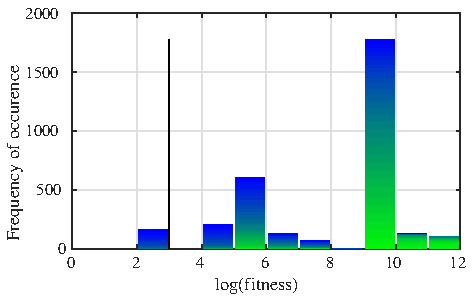
\includegraphics[align=t,smash=br,]{./Bilder/figure_histogram_fitness.pdf}
\input{./Bilder/figure_histogram_fitness_edit.pdf_tex}
\captionof{figure}{Histogram of the fitness function values $f$ of all particles for one optimization of 6\underline{R}RRS with generation highlight.}
\label{fig:histogram_fitness}
\end{figure}
%
A box-plot of the computation time necessary to calculate the fitness function in Fig.\,\ref{fig:boxplot_comptime} proves that the idea of hierarchical constraints works in principle: Particles violating severe constraints are excluded earlier and need less computation time than better solutions.
The box-plots are ordered in classes corresponding to the bars in Fig\,\ref{fig:histogram_fitness}.
The spread in computation times can be explained by the gradient-based inverse kinematics.

\begin{figure}
\centering
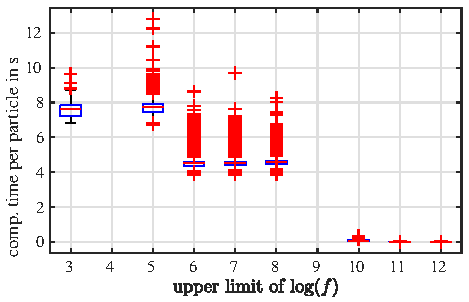
\includegraphics{./Bilder/figure_calctime_vs_fval.pdf}
\vspace{-0.4cm} % Sonst Abstand zwischen Bild und Unterschrift ziemlich groß
\captionof{figure}{Box-plot of computation times of the particles of P6\underline{R}RRS in multiple repetitions corresponding to bars in Fig\,\ref{fig:histogram_fitness}.}
\label{fig:boxplot_comptime}
\end{figure}

\subsection{Evaluation of Condition and Material Stress}
\label{sec:res_matstress}

As elaborated in the introduction, using internal forces and material stress in uncommon in the dimensional synthesis of parallel robots.
Fig.\,\ref{fig:eval_matstress_vs_condition} shows that for the rather lightweight link geometries, the technical limit of the material stress in the final results of multiple runs is nearly reached.
Further, a strong correlation of Jacobian condition number an material stress is not evident, therefore it can be concluded that under the mentioned conditions the consideration of this constraint is useful.

\begin{figure}
\centering
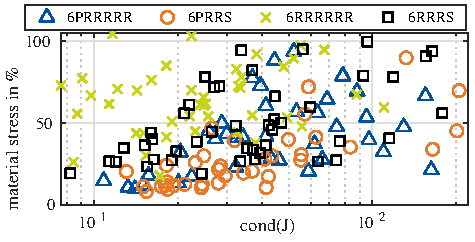
\includegraphics{./Bilder/figure_matstress_vs_condition.pdf}
\vspace{-0.4cm} % Sonst Abstand zwischen Bild und Unterschrift ziemlich groß
\captionof{figure}{Relation of material stress and Jacobian condition number for low tilting angles of about $10^\circ$}
\label{fig:eval_matstress_vs_condition}
\end{figure}



\subsection{Evaluation of Results and Pivoting Angles}
\label{sec:res_condition_pivoting}

The distribution of final results of multiple runs of the optimization is shown in Fig.\,\ref{fig:energy_vs_tiltangle} and Fig.\,\ref{fig:condition_vs_tiltangle} for different maximal tilting angles in the reference trajectory.
The robots with an S-joint seem to perform better than the ones without, as can be summarized from Fig.\,\ref{fig:energy_vs_tiltangle}.

%regarding the objective (consumed energy) in Fig.\,\ref{fig:energy_vs_tiltangle} and the worst condition number during the trajectory in Fig.\,\ref{fig:condition_vs_tiltangle}, which is a common criterion in the dimensional synthesis.

\begin{figure}
\centering
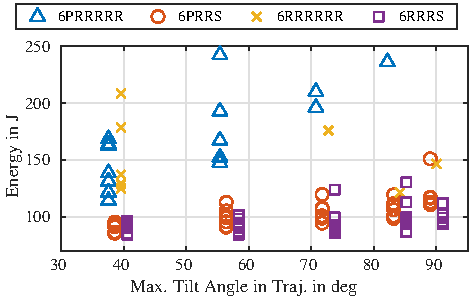
\includegraphics{./Bilder/figure_energy_vs_tiltangle.pdf}
\vspace{-0.4cm} % Sonst Abstand zwischen Bild und Unterschrift ziemlich groß
\captionof{figure}{Comparison of optimization results in different maximum tilt angles of the cube trajectory. Horizontal axes values are shifted from -1.5 to 1.5 for facility of inspection. 9 Repetitions for 4 robots and 5 angles.}
\label{fig:energy_vs_tiltangle}
\end{figure}

On the contrary, the structures with three R-joints instead of one S-joint seem to have a better (lower) condition number in the final results, as can be seen in Fig.\,\ref{fig:condition_vs_tiltangle}.

\begin{figure}
\centering
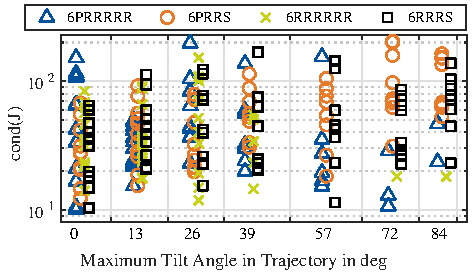
\includegraphics{./Bilder/figure_condition_vs_tiltangle.pdf}
\vspace{-0.4cm} % Sonst Abstand zwischen Bild und Unterschrift ziemlich groß
\captionof{figure}{Worst condition numbers for the results from Fig.\,\ref{fig:energy_vs_tiltangle}}
\label{fig:condition_vs_tiltangle}
\end{figure}



%Neuer Absatz: Detail zu Optimierung
%\begin{itemize}
%\item Die etablierte Partikel-Schwarm-Optimierung zur Lösung des hochdimensionalen Problems der Parameterfindung von Robotern wird hinsichtlich der Behandlung der Nebenbedingungen modifiziert.
%\item Stückweise definierte Fitness-Funktion mit Zielfunktion und Nebenbedingungen als Strafterm hierarchisch, um Rechenzeit zu sparen. Siehe Bild\,\ref{fig:uebersicht}.
%\item Energieverbrauch als Zielfunktion, da skalare Größe gut vergleichbar und andere Zielfunktionen wie Gesamtmasse und damit Dynamik dazu korrelierend
%\end{itemize}

%Neuer Absatz: Kinematik und Dynamik
%\begin{itemize}
%\item Generische Ansätze für inverse Dynamik \cite{DoThanhKotHeiOrt2009b,AbdellatifHei2009} bisher explizit nur für klassische PKM definiert, deren Plattform mit Kugelgelenken verbunden ist
%\item Durch Nutzung von vollständigen Zwangsbedingungen (Position und Orientierung) \cite{Gogu2008,SchapplerTapOrt2019c} einheitlicher Ansatz zum Lösen der inversen Kinematik und der inversen Dynamik möglich.
%\item Durch die Reduzierung des Rechenaufwands ist die Auswertung vieler Parameterkombinationen möglich
%\end{itemize}



\section{Summary and Outlook}
\label{sec:summary}

A general methodology for the modeling and dimensional synthesis of parallel robots is presented, which differs from similar work by being applicable to non-classical parallel robots, the use of a single-objective optimization, the concepts of hierarchical constraints and consumed energy as objective. 
Further work will extend the constraint formulation with considering self-collisions, further plausibility checks and comparing robots with and without task-redundancy and the integration of design optimization of link geometry and drive selection.
%In dem Konferenzvortrag werden die Ergebnisse und der Ansatz der Optimierung im Detail und weitere Beispiele vorgestellt.
%%Dafür wird die Optimierung für weitere Kinematiken und längere Optimierungsdauern durchgeführt sowie statistischen Untersuchungen angestrebt.
%Perspektivisch wird auch die Integration der Entwurfsoptimierung von Antriebs- und Segmentdimensionierung und die Behandlung zusätzlicher Nebenbedingungen und Zielfunktionen diskutiert.

%Als weitere Arbeiten sind Plausibilisierungen hinsichtlich Straftermen für Selbstkollisionen und die Reduktion der Optimierungsparameter geplant.

\section{Acknowledgement}

The authors acknowledge the support by the Deutsche Forschungsgemeinschaft (DFG) under grant OR 196/33-1.

\bibliographystyle{spmpsci_unsrt}
\bibliography{literatur}

%\clearpage  % Verhindert automatischen Umbruch auf der letzten Seite. Bei Bedarf entfernen.


\end{multicols}


\end{document}